
\subsection{AIML Past Paper 2024}
\subsubsection{Question 1}
\begin{enumerate}
    \item[(a)] List the main, formal mathematical elements of a combinatorial optimization problem. [3 marks] \\
    {\color{blue}
    The main formal mathematical elements of a combinatorial optimization problem are: \\
    \begin{math}
    X^\star = \arg\min_{X' \in \mathcal{X}} F(X'). \\
    \end{math}
        A finite set of feasible solutions $\mathcal{X}$. \\
    } 
    \item[(b)] Explain the essential differences between an exact and an approximate algorithm for solving a combinatorial optimization problem. [2 marks] \\
    {\color{blue}
    An exact algorithm guarantees finding the optimal solution to a problem, whereas an approximate algorithm seeks a solution close to the optimum, often with reduced computational effort. Exact algorithms are typically used when precision is critical, and computational resources are sufficient. Approximate algorithms are employed when problems are too complex for exact methods, providing near-optimal solutions more efficiently.
    } 
    \item[(c)] Describe the steps in an exhaustive algorithm for solving an optimization problem. Is this exhaustive algorithm exact or approximate? Justify your answer. [2 marks] \\
    {\color{blue}
    Steps in an exhaustive algorithm:
    \begin{enumerate}
        \item Enumerate all possible configurations in the solution space.
        \item Evaluate the objective function for each configuration.
        \item Select the configuration with the optimal (minimum or maximum) objective value.
    \end{enumerate}
    This exhaustive algorithm is exact because it considers all possible solutions to find the optimal one.
    } 
    \item[(d)] Consider the problem of finding the minimum sum subset of a set of $N$ items.
    \begin{enumerate}
        \item[(i)] What is the size of the configuration space of this problem, in terms of $N$? [1 mark] \\
        \textcolor{blue}{The size of the configuration space is $2^N$, as each item can either be included or excluded from a subset.} 
        \item[(ii)] Give the time complexity class of the exhaustive algorithm for solving this. [1 mark] \\
        \textcolor{blue}{The time complexity class is $\mathcal{O}(2^N)$, since all subsets must be evaluated.} 
        \item[(iii)] Is this exhaustive algorithm tractable or intractable? Justify your answer. [1 mark] \\
        \textcolor{blue}{This exhaustive algorithm is intractable for large $N$ due to its exponential time complexity, making it impractical for large datasets.} 
    \end{enumerate}
    \item[(e)] You are given a set of $N = 3$ items with values $x = [5, -1, 6]$. You must find the minimum sum subset of this set.
    \begin{enumerate}
        \item[(i)] Give the steps in an exhaustive SDP algorithm for solving this problem in $N$ iterations. [5 marks]

\begin{tikzpicture}[
  level distance=2cm,
  sibling distance=2.8cm,
  every node/.style={circle, draw, fill=gray!10, minimum size=0.5cm, font=\small},
  result node/.style={circle, draw, fill=orange!50, font=\small},
  edge from parent/.style={draw, -{Stealth}},
  level 1/.style={sibling distance=6cm},
  level 2/.style={sibling distance=3cm},
  level 3/.style={sibling distance=1.5cm}
]

% Root and first level
\node {[\ ]}
    child {node[result node] {\small [\ ]}
        child {node[] {\small [\ ]}
            child {node[] { [\ ]}}
            child {node[] {\small [6]}}
        }
        child {node[result node] {\small [-1]}
            child {node[result node] { [-1]}}
            child {node[] {\small [-1,6]}}
        }
    }
    child {node {\small [5]}
    % child {node[fill=orange!70] {[X,Y,Z,U]}}
        child {node {\small [5]}
            child {node[] { [5]}}
            child {node[] {[5,6]}}
        }
        child {node {\small [5,-1]}
            child {node[] {[5,-1]}}
            child {node[] {[5,-1,6]}}
        }
    };
% Labels for n levels
\node[anchor=west,draw=none,fill=none] at (7,0) {(initialization, $n=0$)};
\node[anchor=west,draw=none,fill=none] at (7,-2) {$x_1 = 5\ (n=1)$};
\node[anchor=west,draw=none,fill=none] at (7,-4) {$x_2 = -1\ (n=2)$};
\node[anchor=west,draw=none,fill=none] at (7,-6) {$x_3 = 6\ (n=3)$};
\end{tikzpicture}

    {\color{blue}
        \textbf{Initialization:} 
        Initialization: Start with n = 0, generate the root configuration(s) in the set of candidate configurations, S. That is empty. \\
        \textbf{Extensions:}
        Extension: Set n = n + 1, and using data item xn, extend all candidate configurations in S, and append these to S. \\
        \textbf{Reduction:} as previously discussed, the exhaustive approach involves keeping all
possible solutions to the problem, and since every one can be extended to an optimal
configuration, all solutions created during extension will be a candidate configuration.
Therefore, we will not remove configurations at any step; \\
%         Reduction: Remove any candidate configurations from S which cannot be extended to
% an optimal configuration.
        \textbf{Iteration:} Iteration: If n < N, go back to step 2. \\
        \textbf{Select Best:} Select best: Select an optimal configuration $X^\star$ from the remaining candidate configurations
in S. \\
    }
        \item[(ii)] Apply your algorithm to compute the optimal solution, $X^\star$ and its value, $F(X^\star)$, giving the explicit results on each step of your algorithm. [2 marks]
        {\color{blue}
            \begin{itemize}
                \item Subsets and their sums: \\
                    \textbf{1st iteration:} $[]$: $0$ \\
                    \textbf{2nd iteration:} $[]$: $0$ \\
                    \textbf{3rd iteration:} $[-1]$: $-1$ \\
                    \textbf{4th iteration:} $[-1]$: $-1$ \\
                \item The minimum sum is $-1$ for the subset $[-1]$.
                \item Therefore, $X^\star = [-1]$ and $F(X^\star) = -1$.
            \end{itemize}
        }
        \item[(iii)] Now, give a greedy reduction step as part of your SDP algorithm which solves the problem exactly in worst-case linear time, $O(N)$. Justify why this reduction step is valid. [3 marks]
        {\color{blue}
            item The algorithm runs in linear time $\mathcal{O}(N)$ and guarantees finding the minimum sum subset. \\
        }
    \end{enumerate}
\end{enumerate}

\subsubsection{Question 2}
\begin{enumerate}
    \item[(a)] List, provide the usual mathematical symbols, and give the truth tables for, the five basic logical connectives of propositional calculus. [5 marks] \\
    {\color{blue}
    The five basic logical connectives in propositional calculus are:
    \begin{itemize}
        \item Conjunction ($\land$): $P \land Q$ is true if both $P$ and $Q$ are true.
        \item Disjunction ($\lor$): $P \lor Q$ is true if at least one of $P$ or $Q$ is true.
        \item Implication ($\Rightarrow$): $P \Rightarrow Q$ is false only if $P$ is true and $Q$ is false.
        \item Biconditional ($\Leftrightarrow$): $P \Leftrightarrow Q$ is true if $P$ and $Q$ have the same truth value.
        \item Negation ($\lnot$): $\lnot P$ is true if $P$ is false.
    \end{itemize}
    Truth tables:

    \begin{tabular}{|c|c|c|c|c|c|}
    \hline
    $P$ & $Q$ & $P \land Q$ & $P \lor Q$ & $P \Rightarrow Q$ & $P \Leftrightarrow Q$ \\
    \hline
    T & T & T & T & T & T \\
    T & F & F & T & F & F \\
    F & T & F & T & T & F \\
    F & F & F & F & T & T \\
    \hline
    \end{tabular}
    }
    \item[(b)] Translate the following natural language proposition into a formal logical proposition over two propositional variables: “If it is winter but it is not cold, then the climate has changed”. [2 marks] \\
    {\color{blue}
    Let \\
    $W$: "It is winter", \\
    $C$: "It is cold", and \\
    $L$: "The climate has changed". \\
    The proposition translates to: $(W \land \lnot C) \Rightarrow L$.
    }

    \item[(c)] A tautology is a logical proposition which is always true, regardless of the truth value of any propositional variables it uses. Using a truth table, show that the proposition 
    \[
    ((P \Rightarrow Q) \lor R) \lor (P \land \lnot Q \land \lnot R)
    \]
    over the logical variables $P,Q,R$, is a tautology. [5 marks] \\
    {\color{blue}
    To show that $((P \Rightarrow Q) \lor R) \lor (P \land \lnot Q \land \lnot R)$ is a tautology, we construct a truth table:

    \begin{tabular}{|c|c|c|c|c|c|c|c|}
    \hline
    $P$ & $Q$ & $R$ & $P \Rightarrow Q$ & $(P \Rightarrow Q) \lor R$ & $\lnot Q$ & $\lnot R$ & $P \land \lnot Q \land \lnot R$ \\
    \hline
    T & T & T & T & T & F & F & F \\
    T & T & F & T & T & F & T & F \\
    T & F & T & F & T & T & F & F \\
    T & F & F & F & F & T & T & T \\
    F & T & T & T & T & F & F & F \\
    F & T & F & T & T & F & T & F \\
    F & F & T & T & T & T & F & F \\
    F & F & F & T & T & T & T & F \\
    \hline
    \end{tabular}

    Now, compute the final expression:

    \begin{tabular}{|l|r|}
    \hline
    Row & Final Expression \\
    \hline
    1 & T \\
    2 & T \\
    3 & T \\
    4 & T \\
    5 & T \\
    6 & T \\
    7 & T \\
    8 & T \\
    \hline
    \end{tabular}

    Since the final expression is true in all cases, it is a tautology.
    }
    \item[(d)] A simple logical knowledge database contains the following facts: $P =$ “Finley is President”, $Q =$ “Presidents are elected”, along with the rule $R =$ “It is not true that both Finley is President and Presidents are elected”. You must determine whether the query $Y = \lnot P \lor \lnot Q$ is entailed by this database.
    
    \begin{enumerate}
        \item[(i)] Give the steps in the logical model checking algorithm for testing entailment, $R \models Y$ in the given knowledge database. [3 marks] \\
        {\color{blue}
            \textbf{Step 1.List all possible truth assignments for the propositional variables.} \\
            \textbf{Step 2.For each assignment, evaluate the truth value of the premises and the conclusion.} \\
            \textbf{Step 3.If in all cases where the premises are true, the conclusion is also true, then the conclusion is entailed by the premises.} \\
        }
        \item[(ii)] Apply the steps in the model checking algorithm to compute whether $R \models Y$. Show your calculations in full, including any truth tables. [4 marks] \\
        {\color{blue}
        \begin{itemize}
            \item $P$: "Finley is President"
            \item $Q$: "Presidents are elected"
            \item $R$: "It is not true that both Finley is President and Presidents are elected" $\Rightarrow \lnot (P \land Q)$
            \item $Y$: $\lnot P \lor \lnot Q$
        \end{itemize}
        Construct the truth table: \\
        \begin{tabular}{|c|c|c|c|c|c|}
        \hline
        $P$ & $Q$ & $P \land Q$ & $\lnot (P \land Q)$ & $\lnot P \lor \lnot Q$ & $R \Rightarrow Y$ \\
        \hline
        T & T & T & F & F & T \\
        T & F & F & T & T & T \\
        F & T & F & T & T & T \\
        F & F & F & T & T & T \\
        \hline
        \end{tabular} \\
        In all cases where $R$ is true, $Y$ is also true. Therefore, $R \models Y$.
        }
        \item[(iii)] Is this entailment tautological? Justify your answer. [1 mark] \\
        {\color{blue}
        Since the entailment holds in all possible truth assignments, it is tautological.
        }
    \end{enumerate}
\end{enumerate}

\pagebreak
\subsubsection{Question 3}
\begin{figure}
\begin{multicols}{2}
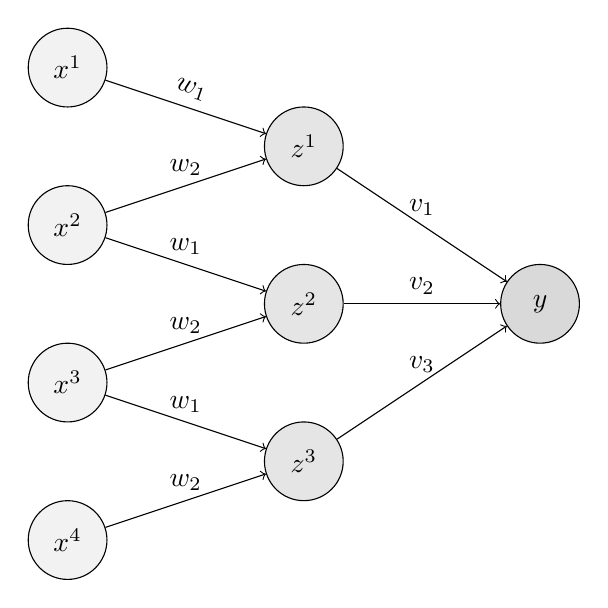
\begin{tikzpicture}[
    node distance=2cm and 5cm,
    neuron/.style={circle, draw, minimum size=10mm},
    input/.style={neuron, fill=gray!10},
    hidden/.style={neuron, fill=gray!20},
    output/.style={neuron, fill=gray!30},
    every edge/.style={->, >=Stealth}
]

% Input layer
\node[input] (x1) at (0,0) {$x^1$};
\node[input] (x2) at (0,-2) {$x^2$};
\node[input] (x3) at (0,-4) {$x^3$};
\node[input] (x4) at (0,-6) {$x^4$};

% Hidden layer
\node[hidden] (z1) at (3,-1.0) {$z^1$};
\node[hidden] (z2) at (3,-3.0) {$z^2$};
\node[hidden] (z3) at (3,-5.0) {$z^3$};

% Output layer
\node[output] (y) at (6,-3) {$y$};

% Connections
\draw[->] (x1) -- (z1) node [midway, above, sloped] (TextNode1) {$w_1$};
\draw[->] (x2) -- (z1) node [midway, above] (TextNode2) {$w_2$};
\draw[->] (x2) -- (z2) node [midway, above] (TextNode3) {$w_1$};
\draw[->] (x3) -- (z2) node [midway, above] (TextNode4) {$w_2$};
\draw[->] (x3) -- (z3) node [midway, above] (TextNode5) {$w_1$};
\draw[->] (x4) -- (z3) node [midway, above] (TextNode6) {$w_2$};

\draw[->] (z1) -- (y) node [midway, above] (TextNode7) {$v_1$};
\draw[->] (z2) -- (y) node [midway, above] (TextNode8) {$v_2$};
\draw[->] (z3) -- (y) node [midway, above] (TextNode9) {$v_3$};

\end{tikzpicture}
    \columnbreak

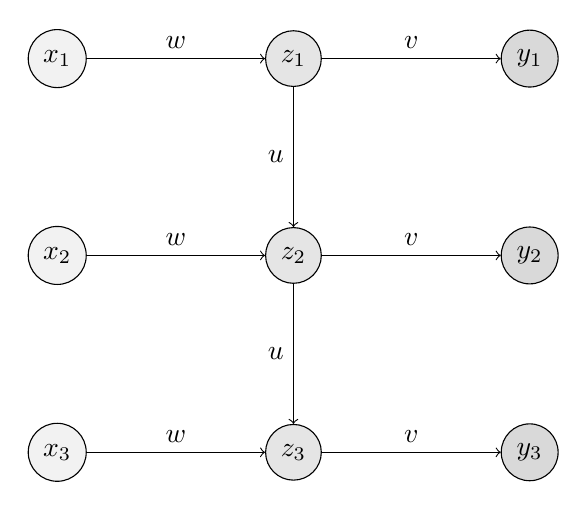
\begin{tikzpicture}[
    node distance=1cm and 1cm,
    neuron/.style={circle, draw, minimum size=7mm},
    input/.style={neuron, fill=gray!10},
    hidden/.style={neuron, fill=gray!20},
    output/.style={neuron, fill=gray!30},
    every edge/.style={->, >=Stealth}
]

% Input layer
\node[input] (x1) at (0,0) {$x_1$};
\node[input] (x2) at (0,-2.5) {$x_2$};
\node[input] (x3) at (0,-5) {$x_3$};

% Hidden layer
\node[hidden] (z1) at (3,0) {$z_1$};
\node[hidden] (z2) at (3,-2.5) {$z_2$};
\node[hidden] (z3) at (3,-5) {$z_3$};

% Output layer
\node[output] (y1) at (6,0) {$y_1$};
\node[output] (y2) at (6,-2.5) {$y_2$};
\node[output] (y3) at (6,-5) {$y_3$};

% Feedforward connections
\draw[->] (z1) to[bend left=0] node[midway,left] {$u$} (z2);
\draw[->] (z2) to node[midway,left] {$u$} (z3);
\draw[->] (x1) to node[midway,above] {$w$} (z1);
\draw[->] (x2) to node[midway,above] {$w$} (z2);
\draw[->] (x3) to node[midway,above] {$w$} (z3);
\draw[->] (z1) to node[midway,above] {$v$} (y1);
\draw[->] (z2) to node[midway,above] {$v$} (y2);
\draw[->] (z3) to node[midway,above] {$v$} (y3);

\end{tikzpicture}
\end{multicols}
\caption{Deep learning networks for Q3.}
\end{figure}

\begin{enumerate}
    \item[(a)] List and provide the mathematical symbols and/or formulae for, three widely used nonlinear activation functions used to construct deep neural networks. [3 marks]
    {\color{blue}
        \begin{itemize}
            \item ReLU (Rectified Linear Unit): $\mathrm{ReLU}(x) = \max(0, x)$
            \item Softplus: $\ln{(1 + e^{x})}$
            \item Hyperbolic Tangent: $\tanh(x) = \frac{e^x - e^{-x}}{e^x + e^{-x}}$
            \item Sigmoid: $\frac{1}{1 + e^{-x}}$
        \end{itemize}
    }
    \item[(b)] For each of the deep neural networks in Figures 1(a) and 1(b) below:
    \begin{enumerate}
        \item[(i)] Identify what is special about the network. [2 marks]
        \item[(ii)] Give an example of the kind of data which would be most suitable for this network to process. [2 marks]
        \item[(iii)] List all the parameters (weights) for the network. [2 marks]
    \end{enumerate}
    {\color{blue}
        \begin{enumerate}
            \item[(i)] 
            \begin{itemize}
                \item \textbf{Figure 1(a):} Fully connected network with a single hidden layer.
                \item \textbf{Figure 1(b):} Layered recurrent structure—each hidden neuron takes input from the current input and the output of the previous neuron.
            \end{itemize}
            
            \item[(ii)] 
            \begin{itemize}
                \item \textbf{Figure 1(a):} Suitable for general-purpose data such as tabular datasets or flattened image vectors.
                \item \textbf{Figure 1(b):} Suitable for time-series or sequential data like speech, text, or sensor readings.
            \end{itemize}

            \item[(iii)]
            \begin{itemize}
                \item \textbf{Figure 1(a):} Weights: $w_{ij}$ between each $x_i$ and $z_j$, and weights $v_j$ between each $z_j$ and output $y$.
                \item \textbf{Figure 1(b):} Parameters include:
                \begin{itemize}
                    \item $w$: input-to-hidden weight,
                    \item $u$: hidden-to-hidden recurrent weight,
                    \item $v$: hidden-to-output weight
                \end{itemize}
            \end{itemize}
        \end{enumerate}
    }
    \item[(c)] For the deep neural network in Figure 1(a), write down the formulae for each of the hidden neurons $z_1, z_2, z_3$ with ReLU nonlinear activation functions, in terms of the inputs $x_1, x_2, x_3, x_4$, and the formula for the output $y$ in terms of the hidden neurons $z_1, z_2, z_3$. [4 marks]
    {\color{blue}

    \begin{math}
    z_1 = \max(0, x_1w_1 + x_2w_2) \\
    z_2 = \max(0, x_2w_1 + x_3w_2) \\
    z_3 = \max(0, x_3w_1 + x_4w_2) \\
    y = \max(0, z_1v_1 +z_2v_2 + z_3v_3) \\
    \end{math}
    }
    \item[(d)] Assume that, for the deep neural network in Figure 1(b), the formulae for computing the values of the hidden and output neurons are:
    \[
    \begin{aligned}
    z_1 &= \max(0, x_1w) &\quad y_1 &= \max(0, z_1v) \\
    z_2 &= \max(0, x_2w + z_1u) &\quad y_2 &= \max(0, z_2v) \\
    z_3 &= \max(0, x_3w + z_2u) &\quad y_3 &= \max(0, z_3v)
    \end{aligned}
    \]
    For the input data $x_1 = 0.3, x_2 = -0.5, x_3 = 1.1$ and where $w = 0.6, u = -0.7, v = 1.5$, compute the values of all hidden and output nodes. Show all your working. [4 marks]

    {\color{blue}
    \begin{math}
    \begin{aligned}
    z_1 &= \max(0,0.3\times0.6)=0.18 &\quad y_1 &= \max(0, 0.18\times 1.5) = 0.27\\
    z_2 &= \max(0,(-0.5)\times0.6 + 0.18\times (-0.7))=0 &\quad y_2 &= \max(0, 0 \times 1.5) = 0 \\
    z_3 &= \max(0,1.1\times0.6 + 0\times)=0.66 &\quad y_3 &= \max(0, 0.66 \times 1.5) = 0.99
    \end{aligned}
    \end{math}
    }

    \item[(e)] Give the diagram for a novel deep network design with two hidden layers, where the first layer is convolutional, the second hidden layer is recurrent, and the last layer is fully connected. Provide unambiguous mathematical labels for all nonlinear nodes and parameters. [3 marks] \\

\begin{tikzpicture}[
  node distance=1.5cm and 1.5cm,
  input/.style={circle, draw=gray, fill=gray!10, minimum size=7mm},
  hidden/.style={circle, draw=gray, fill=gray!10, minimum size=7mm},
  output/.style={circle, draw=green!70!black, fill=green!10, minimum size=7mm},
  ->, >=Stealth
]

% Input
\node[input] (x1) at (0, 6) {$x_1$};
\node[input] (x2) at (0, 3) {$x_2$};
\node[input] (x3) at (0, 0) {$x_3$};

% Conv layer
\node[hidden] (z1) at (3, 4) {$z_1$};
\node[hidden] (z2) at (3, 2) {$z_2$};

% Recurrent layer
\node[hidden] (z3) at (6, 4) {$z_3$};
\node[hidden] (z4) at (6, 2) {$z_4$};

% Output
% \node[output] (y) at (9, 3) {$\hat{y}$};
\node[output] (y) at (9, 3) {$y$};

% Arrows
\draw (x1) to node[near start,above] {$w_1$} (z1);
\draw (x1) to node[near start,below] {$w_2$} (z2);
\draw (x2) to node[near start,above] {$w_1$} (z1);
\draw (x2) to node[near start,below] {$w_2$} (z2);
\draw (x3) to node[near start,above] {$w_1$} (z1);
\draw (x3) to node[near start,below] {$w_2$} (z2);
\draw (z1) to node[near start,below] {$u_1$} (z3);
\draw (z2) to node[near start,below] {$u_2$} (z4);
\draw (z3) to node[near start,below] {$v$} (z4);
\draw (z3) to node[near start,below] {$t_1$} (y);
\draw (z4) to node[near start,below] {$t_2$} (y);

\node[anchor=west,draw=none,fill=none] at (0,-1) {input};
\node[anchor=west,draw=none,fill=none] at (2,-1) {first layer};
\node[anchor=west,draw=none,fill=none] at (5,-1) {second layer};
\node[anchor=west,draw=none,fill=none] at (7.5,-1) {last layer(output)};
\end{tikzpicture}

%\textbf{Mathematical labels:}
% \[
% \begin{aligned}
% Z &= \sigma(W_c * X) \\
% H_t &= \sigma(W_r Z_t + U H_{t-1}) \\
% \hat{y} &= \phi(V H)
% \end{aligned}
% \]

% Where:
% \begin{itemize}
%     \item $W_c$: convolution filter parameters
%     \item $W_r$, $U$: recurrent weights
%     \item $V$: weights for final dense layer
%     \item $\sigma$, $\phi$: activation functions (e.g., ReLU, softmax)
% \end{itemize}

\end{enumerate}
